% ============================================================
% Q2 – Named Entity Recognition
% ============================================================
\section{Question 2 -- Named Entity Recognition}

\subsection{Dataset: CoNLL-2003}

The CoNLL-2003 English NER dataset~\cite{tjong2003conll} annotates newswire text
with four named entity types using the BIO scheme:

\begin{table}[H]
  \centering
  \caption{CoNLL-2003 Entity Types and BIO Tagging}
  \label{tab:q2_tags}
  \begin{tabular}{llr}
    \toprule
    \textbf{Prefix} & \textbf{Entity} & \textbf{Tag IDs} \\
    \midrule
    B-PER / I-PER  & Persons        & 1, 2 \\
    B-ORG / I-ORG  & Organisations  & 3, 4 \\
    B-LOC / I-LOC  & Locations      & 5, 6 \\
    B-MISC / I-MISC & Miscellaneous  & 7, 8 \\
    O               & Outside        & 0 \\
    \bottomrule
  \end{tabular}
\end{table}

\begin{figure}[H]
  \centering
  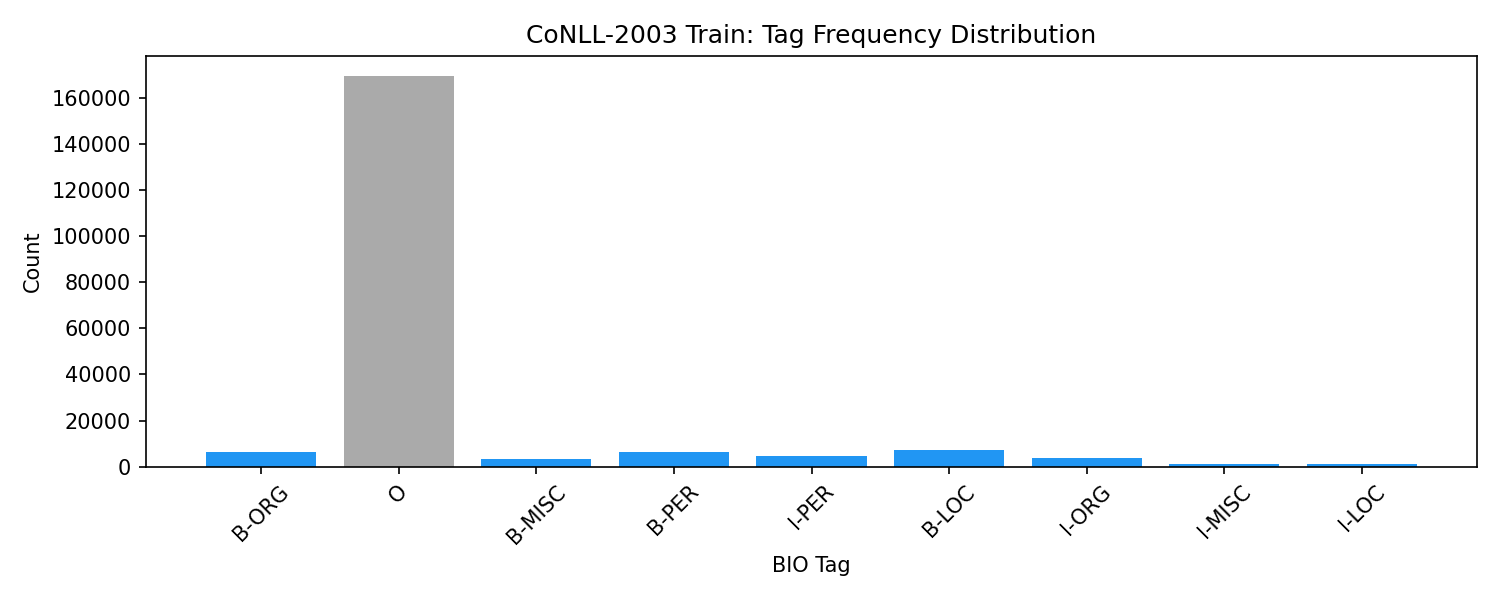
\includegraphics[width=0.75\textwidth]{figures/conll_tag_dist.png}
  \caption{CoNLL-2003 training set: BIO tag frequency distribution.}
  \label{fig:conll_tag_dist}
\end{figure}

\noindent\textbf{BIO alignment for subword tokenisers.}
When WordPiece splits a word into multiple subword tokens, only the
\emph{first subword} of each word receives the gold label; continuation
subwords are masked with \texttt{-100} and excluded from loss and evaluation.

\subsection{Models}

\subsubsection{Model 1 -- BiLSTM-CRF}

A 2-layer bidirectional LSTM (hidden=128/direction) feeds a Conditional Random
Field (CRF) decoding layer (\texttt{pytorch-crf}).
The CRF learns \emph{transition probabilities} between tags, globally
enforcing valid BIO sequences (e.g., \texttt{I-PER} cannot follow \texttt{B-ORG}).
Vocabulary: 100-dim random embeddings, min-freq=1.

\subsubsection{Model 2 -- BERT-base-cased (Fine-tuned)}

\texttt{bert-base-cased}~\cite{devlin2019bert} is used (cased is critical for NER — capitalisation
is a strong signal for entity recognition). A linear classification head
(768 $\to$ 9) is added atop the last hidden states.
Fine-tuned with $\text{lr}=2\times10^{-5}$, batch=16, 3 epochs.

\subsection{Results}

\begin{table}[H]
  \centering
  \caption{NER Evaluation on CoNLL-2003 Test Set (entity-level, \texttt{seqeval})}
  \label{tab:q2_results}
  \begin{tabular}{lccc}
    \toprule
    \textbf{Model} & \textbf{Precision} & \textbf{Recall} & \textbf{F1} \\
    \midrule
    BiLSTM-CRF     & 0.6999 & 0.6710 & 0.6852 \\
    BERT-base-cased & 0.9041 & 0.9187 & 0.9113 \\
    \bottomrule
  \end{tabular}
\end{table}

\begin{figure}[H]
  \centering
  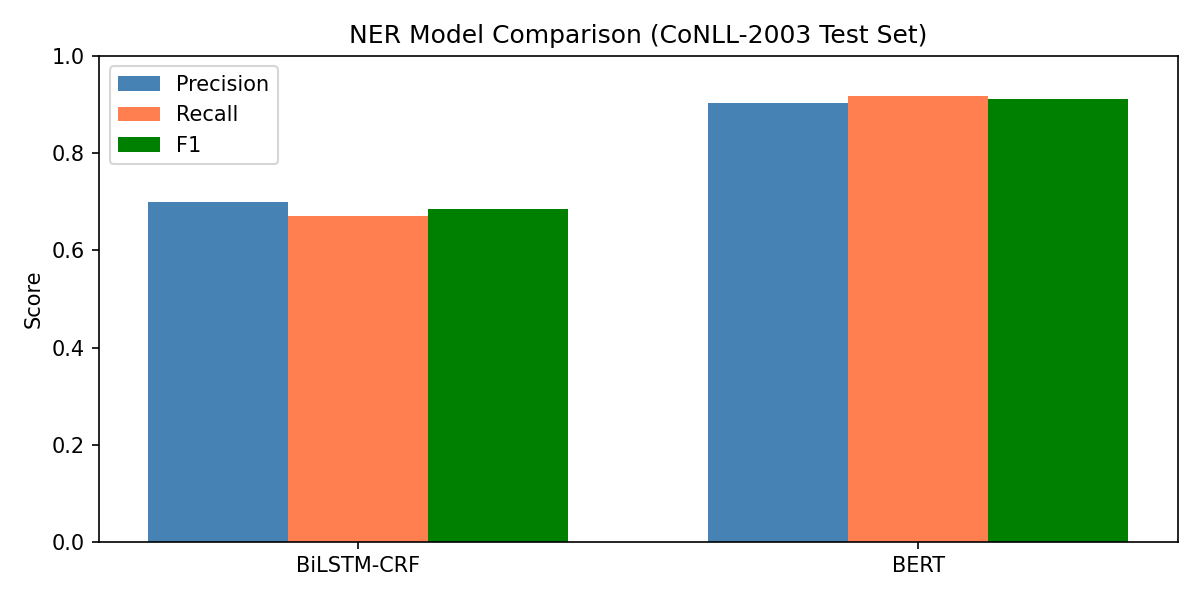
\includegraphics[width=0.65\textwidth]{figures/ner_comparison.png}
  \caption{NER model comparison: Precision, Recall, and F1 on the CoNLL-2003 test set.}
  \label{fig:ner_comparison}
\end{figure}

\subsection{Error Analysis}

\begin{description}[leftmargin=1.5em]
  \item[Boundary errors] Both models misplace B-/I- prefix transitions.
    Example: ``New York City'' predicted as \texttt{B-LOC B-LOC I-LOC}
    instead of \texttt{B-LOC I-LOC I-LOC}.
  \item[Entity type confusion] Ambiguous tokens such as \textit{Washington}
    (person, city, or organisation) frequently confuse entity type assignment.
  \item[O $\to$ MISC miss] Short, rare MISC entities are often left undetected,
    lowering recall for this class.
  \item[BiLSTM-CRF unseen words] Token not in training vocabulary collapse to
    \texttt{<unk>}, losing surface-form information that BERT preserves via subword splitting.
\end{description}

\begin{figure}[H]
  \centering
  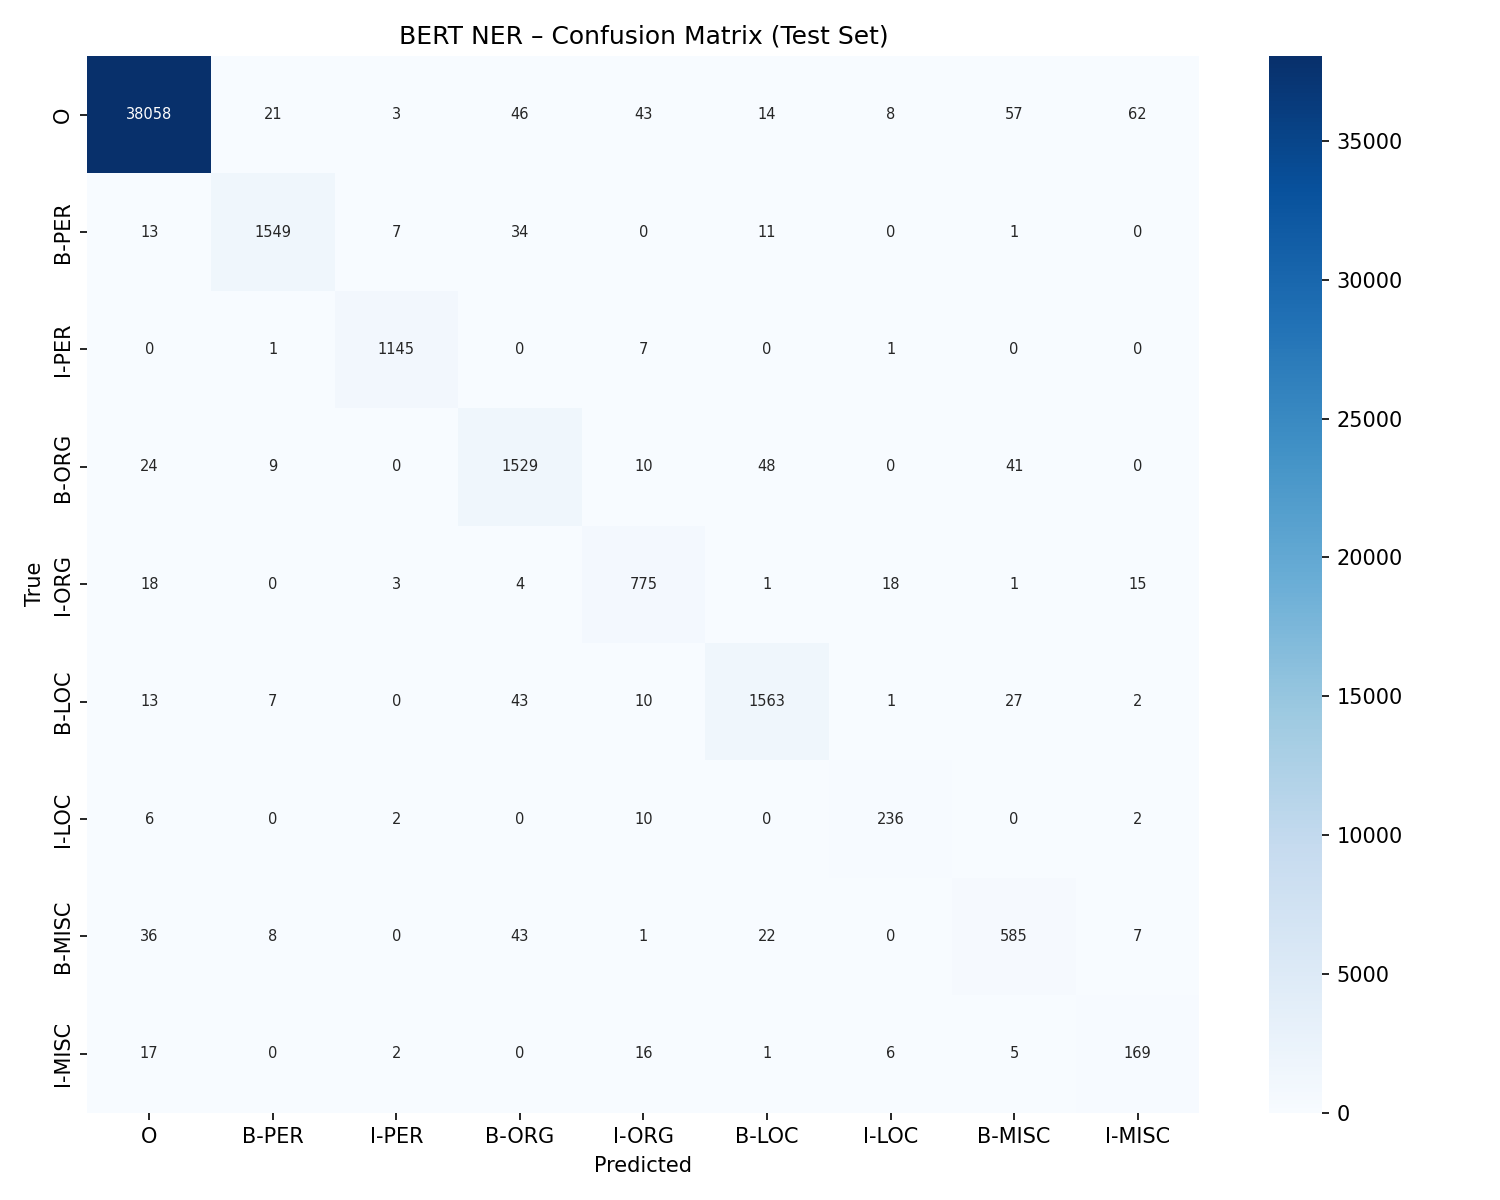
\includegraphics[width=0.75\textwidth]{figures/ner_bert_confusion.png}
  \caption{BERT NER confusion matrix on the CoNLL-2003 test set (token-level).}
  \label{fig:ner_bert_conf}
\end{figure}

\subsection{Discussion: Role of Contextual Embeddings}

BERT's pre-trained contextual representations capture long-range syntactic and
semantic context unavailable to the LSTM.
The cased BERT model preserves capitalisation patterns, a decisive signal for
entity recognition.
The CRF layer in BiLSTM-CRF enforces global BIO consistency, reducing boundary
errors compared to a plain softmax head; however, BERT's richer representations
more than compensate, achieving higher F1 without explicit CRF decoding.
